\section{Validation and measured performance}
\label{sec:measurements}

The evidence has three different roles. Exhaustive small matrices test the
algebra against an independent search over all permitted pivots. Genuine
normal cuts test source compilation and the geometric census. Paired timing
experiments measure the cost of particular implementations. None of these
finite experiments proves the general theorems; their proofs appear above.
The exact inputs, raw samples, logs and source hashes are supplied with
this article, as described in Appendix~\ref{sec:reproduction}.

\subsection{Algebraic and certificate validation}

The column-cancellation tests enumerate every legal saturated positive-pivot
schedule on 31,096 small matrices and compare full success with both the
new source peeling and the retained capped planner. All agree. A further
350 seeded random matrices are checked against every row-subset stopping
condition and the permanent-one-minor characterization. These tests include
rectangular inputs, zero rows, coefficients two, and incomplete prefixes.
The explicit 4,000-row chain test records exactly 8,000 source-incidence
visits and zero fill updates.

The seven new column-cancellation test methods are included in a focused
36-test run with the existing core, whole-cut, primitive-annulus and
disk-absorption tests. All 36 pass. Certificate tests cover duplicate
pivots, nonexistent and Boolean labels, malformed counts, altered
certificates, large integers, prefix checking and caller aborts.

The saturated extension adds 17 focused tests, all passing. They include
native geometric sources, independent replay with the producers disabled,
altered port charts, exact binary/hexadecimal transport, budget exhaustion,
and callback propagation. Negative controls include the aggregate-two
annulus and the winding-three M\"obius attachment described above. An
abstract finite interface model takes base genus
\[
 q=2^{16384}+17
\]
and obtains genus $2q$ using one aggregate incidence. This checks the
implementation's refusal to expand numerical genus and its exact integer
transport. It is a conditional finite-model test, not a claim that a new
native triangulation realizing that particular huge-genus source was
constructed during this study.

The passenger extension has ten additional tests. An independent oracle
performs the full positive update on all remaining rows, rather than
using immutable donors. It examines all 729 ternary $2\times3$ donor
matrices and 8,748 candidate complete schedules; the 324 valid schedules
agree exactly. There are also 120 randomly relabelled acyclic examples,
branching and merging paths, passenger-only columns, empty cases, and
uncapped counts exceeding 8,192 bits. Invalid schedules are rejected.

The maintained suite run completed \textbf{1,687 tests in 365.654 seconds},
all passing. The passenger module was added after that run's collection
and was tested separately: all ten tests passed. A final collection-only
check counts 1,697 tests in the delivered source tree. Thus the reported
validation is one complete 1,687-test run plus the ten new isolated tests,
not a claimed second full 1,697-test execution. The maintained run also
reports 13,846 expanded-sheet topology comparisons and its independent
marked-cover audit; the full output is retained verbatim.

\subsection{The pinned source corpus and unchanged core coverage}

The retained corpus consists of 106 supplied normal cuts, including layered
solid-torus cases, mixed coordinates, source relabellings, other finite
triangulations and large binary coordinate families. Its exact JSON has
SHA-256
\begin{center}\small
\path{97b4ceed6f068885760d80dea214538634998dd405b77e76926c1f93db03da5c}.
\end{center}
Every experiment names the repository pin. The saved old primitive-annulus
audit is also hashed. This corpus is a retained regression collection,
not a random sample of knots and not a performance distribution for
crossing number $n$.

On prepared source cores, the new producer follows these paths:
\begin{center}
\begin{tabular}{@{}lr@{}}
\toprule
Core outcome or certificate path & Cases\\
\midrule
Existing square row-leaf success & 66\\
New column-leaf certificate path & 24\\
Raw-cancellation stall & 6\\
Core three-handle exclusion & 10\\
\bottomrule
\end{tabular}
\end{center}
The 24 column-path successes were already successes of the old capped
planner. Both produce 90 successful core results. Substituting the new
core producer into the existing whole-cut consumer gives exactly the
same 78 complete censuses and 28 inconclusive results as before; all
156 successful old/new whole-cut certificates independently replay.
This confirms the acceptance-class correction proved in
Proposition~\ref{prop:old-complete}.

\subsection{Paired timing protocol and synthetic scaling}

The benchmark retains exact copies of the old producer and verifier from
the pinned commit. It alternates execution order over five paired trials,
uses a preliminary measurement to choose a small repeat count for each
side, divides by that repeat count, and reports the median per call.
The ratio is the baseline median divided by the new median. Raw samples,
repeat counts and operation counters are in the delivered JSON.

The recorded environment is CPython 3.12.14 on Linux 6.18.44, x86\_64,
with glibc 2.39. The experiments used the shared research runtime; they
are not hardware-isolated microbenchmarks or statistical confidence
intervals. Their strongest asymptotic evidence is the source-operation
count, alongside the proved bound.

For the bidiagonal family $N_m$ of Section~\ref{sec:algorithms}, the old
planner records $2m(m+1)$ source-entry scans and the new planner $2m$
incidence visits. Both perform zero fill updates. The measured producer
medians are:
\begin{center}
\begin{tabular}{@{}rrrrr@{}}
\toprule
Rows $m$ & Nonzeros & Baseline (ms) & New (ms) & Ratio\\
\midrule
16 & 32 & 0.1074 & 0.0190 & $5.67\times$\\
64 & 128 & 1.4318 & 0.0764 & $18.73\times$\\
256 & 512 & 20.1221 & 0.5037 & $39.95\times$\\
1,024 & 2,048 & 552.0291 & 2.3910 & $230.88\times$\\
4,096 & 8,192 & 7,456.9916 & 7.2578 & $1,027.45\times$\\
\bottomrule
\end{tabular}
\end{center}

\begin{figure}[htbp]
\centering
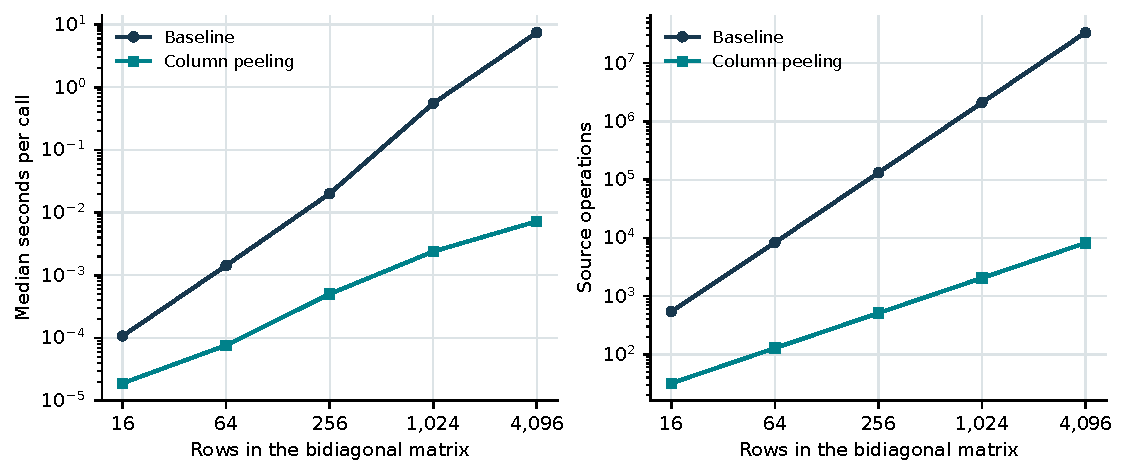
\includegraphics[width=\textwidth]{figures/cancellation_scaling.pdf}
\caption{The measured bidiagonal cancellation family. Left: five-trial
median producer times. Right: exact source-operation counters. Both axes
are logarithmic. The curves connect measured points; they are not fitted
claims about the full recognizer. The figure is regenerated directly
from the supplied benchmark JSON.}
\label{fig:scaling}
\end{figure}

The synthetic replay experiment uses conditional core incidence words,
not authenticated embedded three-dimensional sources. At 256 rows its
old median is 729.837 ms and its new median is 0.776 ms, a ratio of
$939.98\times$. This shows the cost removed by immutable timestamp replay
in the intended finite checker. It does not measure source authentication.

\subsection{Native timing: a small-kernel regression and almost unchanged queries}

The source-backed timing experiment separates prepared finite cores from
the entire old whole-cut query:
\begin{center}
\begin{tabular}{@{}p{.43\textwidth}rrr@{}}
\toprule
Scope & Baseline & New & Ratio\\
\midrule
All 106 prepared core producers & 4.807 ms & 6.515 ms & $0.738\times$\\
The 24 affected core producers & 1.397 ms & 0.974 ms & $1.435\times$\\
All 90 successful core replays & 7.084 ms & 5.703 ms & $1.242\times$\\
Complete 106-case old cut query & 36.515 s & 36.211 s & $1.008\times$\\
\bottomrule
\end{tabular}
\end{center}

The aggregate prepared-core timing is a regression: the new median is
about 35.6\% larger. This result must remain visible alongside the affected
subset's improvement. The samples vary, and such small calls are sensitive
to runtime overhead. The retained fast row-leaf path helps preserve
compatibility, but the data do not support a universal practical speedup.

The complete-query medians are effectively unchanged. Source orbit
construction, boundary observation and other work remain substantial;
the raw finite planner is too small a fraction of this corpus's full
query cost to transform the total. The synthetic thousand-fold ratio
must therefore not be advertised as an unknot-recognition speedup.
A next performance study should target authenticated source-query reuse
and boundary observation, while preserving this paired full-query scope.

\subsection{Seven additional geometric successes}

The saturated-bundle operator addresses coverage rather than simply
substituting a faster planner. Its final independent audit has the
following outcomes:
\begin{center}
\begin{tabular}{@{}lr@{}}
\toprule
Audit quantity & Count\\
\midrule
Supplied cuts & 106\\
Complete new whole-cut censuses & \textbf{85}\\
Earlier complete censuses retained & 78 of 78\\
New complete censuses & 7\\
Independent source-certificate replays & 85 of 85\\
Fresh Regina literal cuts completed & 99\\
Successful source censuses within literal-cut cap & 78\\
Agreement on those successful censuses & 78 of 78\\
Large-coordinate successes replayed without expansion & 7\\
Remaining joint raw stalls & 11\\
Remaining three-handle exclusions & 10\\
\bottomrule
\end{tabular}
\end{center}

All seven new cases previously returned \code{annular_core_attachment}.
All seven admit fresh literal cuts in Regina 7.4, and those independently
computed censuses agree with the new source proof. The seven successful
large-coordinate cases beyond the literal expansion cap are distinct
from these seven new cases; they are independently replayed but are not
claimed to have fresh expanded Regina comparisons.

In the following table $b$ is the number of base boundary components.
The listed genera are for the whole cut, with repeats indicating distinct
components. Genus zero denotes a ball.
\begin{center}\small
\begin{tabular}{@{}p{.39\textwidth}rlc@{}}
\toprule
Case & $T$ & Saturated nondisk base & Cut genera\\
\midrule
\path{pilot/fibonacci_lst_05/0} & 5 & M\"obius, $(\chi,b)=(0,1)$ & $1,2$\\
\path{pilot/fibonacci_lst_07/0} & 7 & M\"obius, $(0,1)$ & $1,2$\\
\path{pilot/fibonacci_lst_09/0} & 9 & M\"obius, $(0,1)$ & $1,2$\\
\path{pilot/lst_4_7/0} & 4 & M\"obius, $(0,1)$ & $1,2$\\
\path{pilot/lst_7_10/0} & 5 & M\"obius, $(0,1)$ & $1,2$\\
\path{fibonacci_lst_09/mixed} & 9 & One crosscap, $(-1,2)$ & $0,3,3$\\
\path{fibonacci_lst_10/mixed} & 10 & Annulus, $(0,2)$ & $0,2,2$\\
\bottomrule
\end{tabular}
\end{center}

The entire audit, including fresh oracle subprocesses, took 86.04 seconds.
That is a single mixed validation run, not a paired speed comparison
with the prior consumer. The package retains every case outcome,
refusal reason, source hash and fresh-oracle result. All 21 unresolved
cases remain inconclusive.

\subsection{Explicit witnesses for the remaining raw stalls}

The package also extracts all eleven remaining joint stopping sets.
For each case, the parallelity and boundary source proofs independently
replay before the exact matrix is read, and the separate obstruction
checker verifies the resulting nonempty row set. Six cases already have
an obstruction in their original-core row submatrix. In the other five,
that submatrix fully cancels and the obstruction requires the added
saturated relations. All five of those latter cases have saturated disk
bases, so the unresolved compatibility is already present in the
disk-absorption subproblem.

For example, \path{solid_torus_sum_rp3/mixed} has the stopping rows
$(8,10,11)$ on its nonzero stopping columns $(8,28,32)$, with matrix
\[
 \begin{pmatrix}2&1&1\\0&1&0\\0&0&1\end{pmatrix}.
\]
Every column sum is two. Its original-core row submatrix nevertheless
admits a full raw schedule. This small source witness makes the joint
compatibility issue concrete. It certifies a raw obstruction; it does
not infer the topology of that cut from an unsigned determinant or
from the triangulation's example name.

Exact uncapped matrices, row ownership, canonical stopping sets,
source-proof hashes and the old-core comparison are retained in
\path{artifacts/saturated/stopping_obstructions.json}. A portable
extractor reproduces them. These witnesses make the next investigation
of refused cases reproducible, while keeping unsupported topological
conclusions separate from algebraic ones.

\subsection{A complete small source example}

The smallest new example is \path{pilot/lst_4_7/0}. Its triangulation has
isomorphism signature \code{eHKPbcddhqxr} and four tetrahedra. Its normal
coordinates, in the source's seven-coordinate order per tetrahedron, are
\[
\begin{pmatrix}
1&1&1&1&0&0&0\\
1&1&1&1&0&0&0\\
1&1&0&0&1&0&0\\
0&0&0&0&0&2&0
\end{pmatrix}.
\]
The new saturated base is profile 0, a M\"obius band with one fully
attached annulus. It contributes one virtual band and relation row 5.
On original nonforest columns $(4,12,14,15,18,19,20,21)$, the exact
aggregate matrix, in row order $0,\ldots,5$, is
\[
 A=\begin{pmatrix}
 0&0&0&1&1&0&0&0\\
 0&0&0&0&0&1&0&0\\
 0&0&1&0&1&0&1&1\\
 0&0&0&1&0&1&1&1\\
 0&0&0&0&1&0&1&0\\
 1&2&0&0&0&0&0&0
 \end{pmatrix}.
\]
The omitted bundle column contains two in row 5 and zero in every other
row. The first five rows are the original core relations; they already
admit full cancellation when considered alone.
The verified source row/column schedule is
\[
(2,14),\ (5,4),\ (3,21),\ (0,15),\ (4,20),\ (1,19).
\]
The result consists of two components, of genera two and one. Their
Euler characteristics are $-1$ and $0$, summing to $-1$. Relation 5 is
cancelled at the second step using an old core column, while its virtual
band never appears in the stored matrix. This illustrates the exact
mechanism of the geometric extension on a genuine input.

The complete labelled tetrahedron gluings, source proofs, forest,
boundary charts, finite certificate and normal vector are in
\path{artifacts/saturated/certificates/019.json}. They determine the
source even if a different triangulation labelling is produced from
the isomorphism signature. The other six cases are recorded at the same
level of detail, rather than only by an expected genus or an example name.
